\documentclass[11pt]{article}

\usepackage{acl2013}
\usepackage{times}
\usepackage{latexsym}
\usepackage{amsmath}
\usepackage{multirow}
\usepackage{array}
\usepackage{url}
\usepackage{graphicx}
\usepackage{subfig}
\usepackage{marvosym}
\usepackage{todonotes}

\setlength\titlebox{6.5cm}

\newcommand{\mnote}[1]{\marginpar{%
  \vskip-\baselineskip
  \raggedright\footnotesize
  \itshape\hrule\smallskip\footnotesize{#1}\par\smallskip\hrule}}

%% \newcommand{\aff}{\ensuremath{{}^\text{\Radioactivity}}}
%% \newcommand{\afff}{\ensuremath{{}^\text{\Bat}}}
\newcommand{\hltcoe}{\ensuremath{{}^\text{1}}}
\newcommand{\clsp}{\ensuremath{{}^\text{2}}}
\newcommand{\upenn}{\ensuremath{{}^\text{2}}}
\newcommand{\grammarrule}[3]{$#1 \to \langle \text{#2} , \text{#3} \rangle$ }

\title{Joshua 5.0: Every day, and in every way, getting better and better}

\author{Matt Post\hltcoe \and Juri Ganitkevitch\clsp \and Yuan Cao\clsp \and Jonathan Weese\clsp 
  \and Luke Orland\hltcoe \\
  \clsp Center for Language and Speech Processing \\
  \hltcoe Human Language Technology Center of Excellence \\
  Johns Hopkins University \\
  Baltimore, MD 21218
  \AND  Chris Callison-Burch \\
  Computer and Information Sciences Department \\
  University of Pennsylvania \\
  Philadelphia, PA 19104
}

\date{}

\begin{document}
\maketitle

\begin{abstract}
  We describe improvements made over the past year to Joshua, an
  open-source translation system for parsing-based translation. The
  main contributes this past year are significant improvements in
  speed and usability of the grammar extraction and decoding steps. We
  have also extended Joshua with support for sparse features and
  training of large numbers of features with discriminative training
  methods.
\end{abstract}

%%%%%%%%%%%%%%%%%%%%%%%%%%%%%%%%%%%%%%%%%%%%%%%%%%%%%%%%%%%%%%%%%
\section{Introduction}
\label{sec-intro}

Joshua is an open-source toolkit\footnote{\url{joshua-decoder.org}}
for parsing-based statistical machine translation of human languages.
The original version of Joshua \cite{Joshua-WMT} was a port (from
Python to Java) of the Hiero machine translation system introduced by
\newcite{Chiang2007}.  It was later extended to support grammars with
rich syntactic labels \cite{li2010joshua}. Subsequent efforts produced
Thrax, the extensible Hadoop-based extraction tool for synchronous
context-free grammars \cite{Joshua-3.0}, which was later extended to
support pivoting-based paraphrase extraction \cite{Joshua-4.0}.

Here are a summary of the major components of Joshua 5.0:

\begin{itemize}
  \item \emph{Sparse features}. Joshua now supports an
    easily-extensible sparse feature implementation, along with tuning
    methods (PRO and KBMIRA) for efficiently setting the weights on
    large feature vectors.
  \item \emph{Significant speed increases}. Joshua 5.0 is up to six
    times faster than Joshua 4.0 and three times faster than
    hierarchical Moses.
  \item \emph{Thrax 2.0}. A reengineered Thrax is up to 300\% faster
    while using significantly less intermediate disk space.
  \item \emph{Many other features} including a server mode with fair
    round-robin schedule among and within requests, pipeline
    improvements, and better end-user documentation.
\end{itemize}

%%%%%%%%%%%%%%%%%%%%%%%%%%%%%%%%%%%%%%%%%%%%%%%%%%%%%%%%%%%%%%%%%
\section{What's New in Joshua 5.0}

\subsection{Sparse features}

%% Until a few years ago, machine translation systems were for the most
%% part limited in the number of features they could employ, since the
%% line-based tuning method, MERT \cite{Och2003}, was not able to
%% efficiently search over more than a few tens of feature weights. The
%% introduction large-scale discriminative tuning procedures has made it
%% possible to tune thousands of parameters simultaneously. With so many
%% features, many of them binary, it becomes important to be able to
%% represent them internally in an efficient manner.

The introduction of discriminative tuning methods for machine
translation \cite{liang2006end,chiang2008online,PRO2011} has made it
possible to tune large numbers of features in statistical machine
translation systems, and open-source implementations have made it easy
\cite{cherry2012batch}.  When dealing with large numbers of features
(on the order of thousands), it is important that they be represented
in a sparse format, particularly since large feature sets often employ
many binary-valued features, a large number of which are zero for any
particular edge in the hypergraph.

Joshua 5.0 has moved to a sparse feature representation
internally. Terminologically, features are instantiated as
\emph{templates}, each of which can contribute any number of features
to the decoder. For example, the (typically dense) features stored
with the grammar on disk are each separate features contributed by the
\textsc{PhraseModel} feature function template. The
\textsc{LangaugeModel} template contributes only a single feature
value for each language model that was loaded (typically one).

Adding new sparse features is as easy as implementing the following
(simplified) interface:
%
\begin{itemize}
\item \texttt{computeCost(edge, i, j)} Returns the cost of applying a
  rule (an edge in the hypergraph).
\item \texttt{computeFeatures(edge, i, j)} Computes the features fired
  when applying a rule.
\end{itemize}
%
At each n-ary rule application, all features are asked to score the
rule.  For performance reasons, during construction of the chart, each
feature only needs to contribute a scalar value of the inner product
of the weight vector and the features incurred on that hyperedge. The
actual feature names and values need not be explicitly represented
unless that information is requested during k-best extraction.

For tuning large sets of features, Joshua supports both PRO
\cite{PRO2011} (introduced with Joshua 4.0) and k-best batch MIRA
\cite{cherry2012batch}.

The sparse feature implementation did not result in increased decoding
speeds and, in fact, is part of a large performance increase in
Joshua, which we now describe.

\subsection{Performance improvements}

We introduced many performance improvements, replacing code designed
to get the job done under research timeline constraints with more
efficient alternatives. The details are outside the scope of this
paper, but include smarter handling of locking across threads, more
efficient (non string-based) computation of dynamic programming state,and
replacement of fixed class-based array structures with literals.

We used the following experimental setup to compare Joshua 4.0 and
5.0: We extracted a large German-English grammar from all sentences
with no more than 50 words per side from Europarl v.7 and the Common
Crawl data using Thrax default settings.  After filtering against our
test set, this grammar contained 70 million rules.  We then trained
three language models on (1) the target side of our grammar training
data, (2) English Gigaword, (3) the monolingual English data released
for WMT13. We tuned a system using KBMIRA and decoded using KenLM
\cite{KenLM}.  Decoding was performed on 64-core 2.1 GHz AMD Opteron
processors with 256 GB of available memory.

Figure~\ref{fig:cmp} Figure~\ref{fig:cmp} plots the minimum end-to-end
runtime\footnote{i.e., including model loading time and grammar
  sorting.} as a function of the number of threads.  Each point in the
graph is the minimum of at least fifteen runs computed at different
times over a period of a few days.  Joshua 5.0 is up to 500\% faster
than it was last year, especially in multithreaded situations.

\begin{figure}[!t]
  \begin{center}
    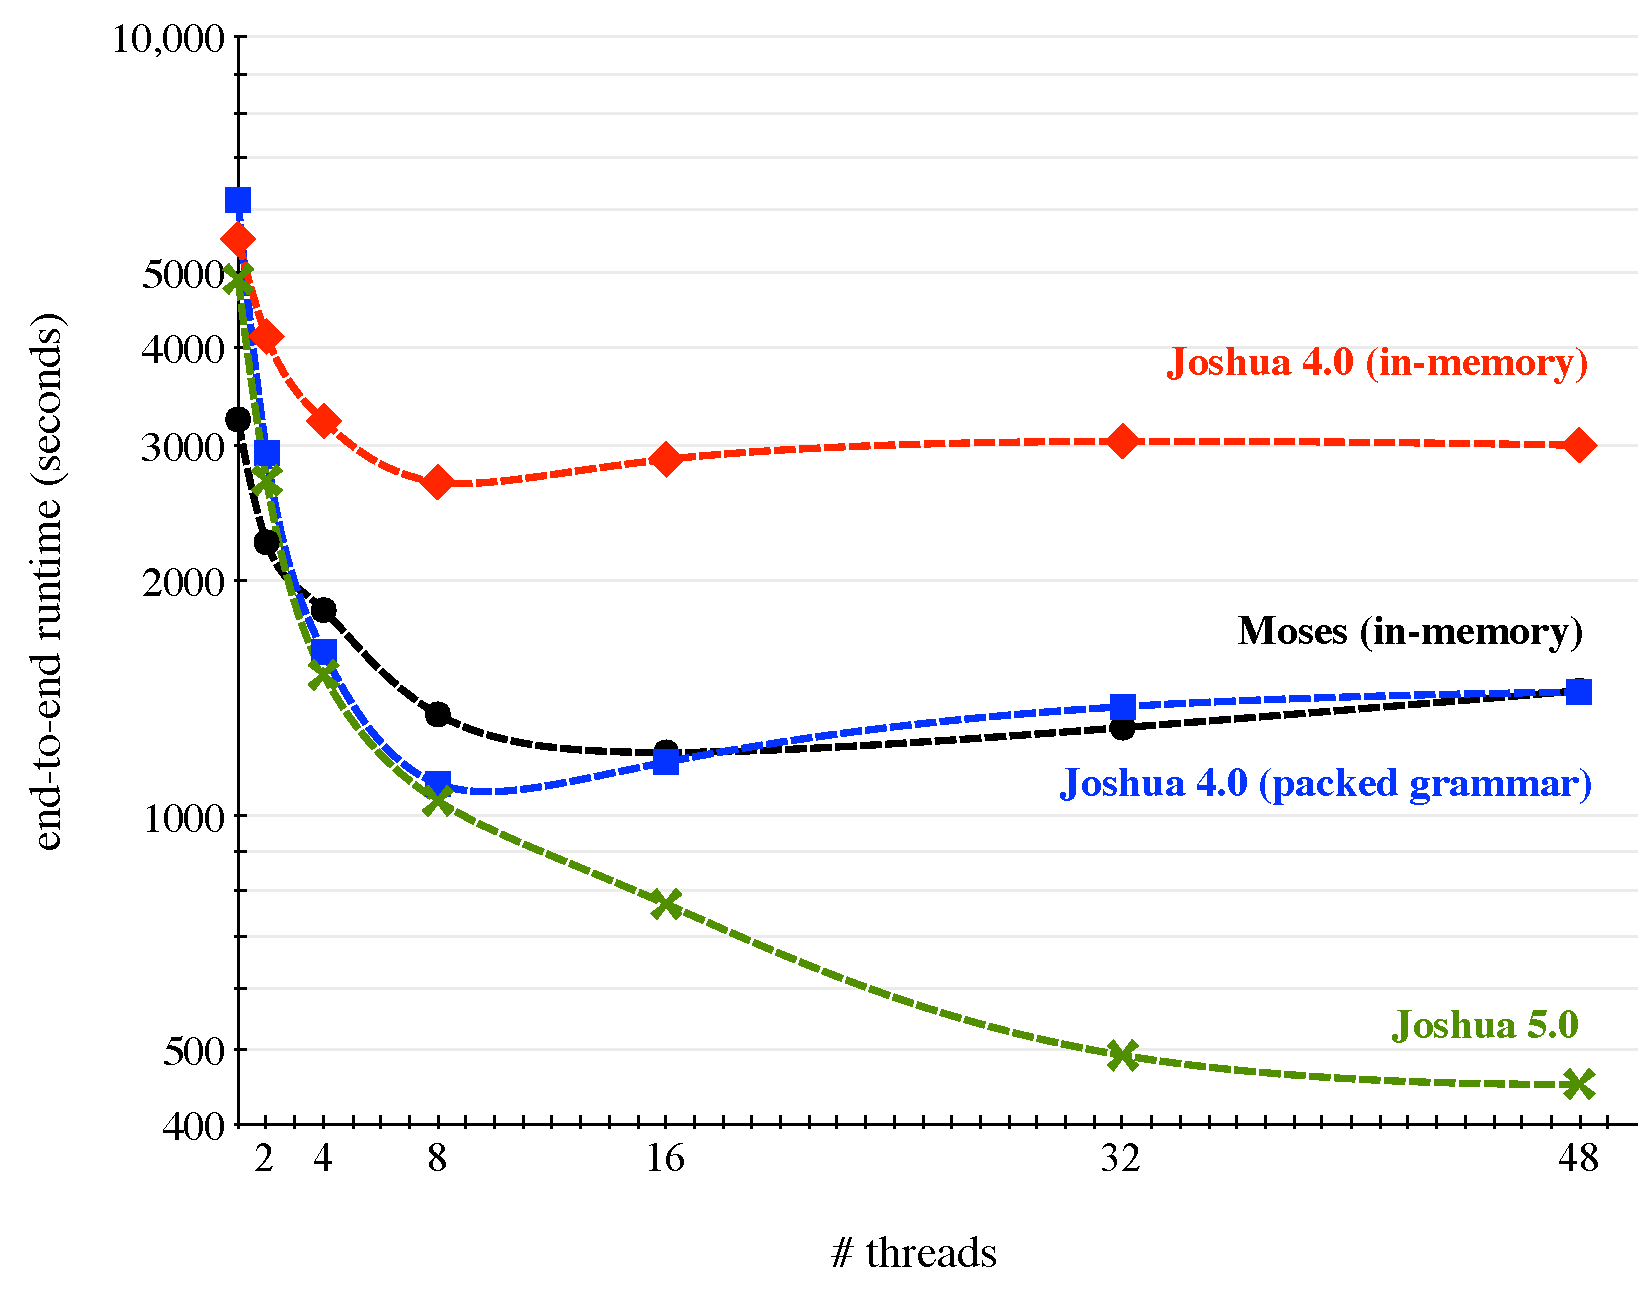
\includegraphics[width=0.99\linewidth]{figures/comparison.pdf}
  \end{center}
  \label{fig:cmp}
  \caption{End-to-end runtime as a function of the number of threads
    for Joshua 4.0 and Joshua 5.0 and Moses. Each data point is the
    minimum of at least fifteen different runs taken at different
    times over multiple days.}
\end{figure}

For further further comparison, we took these models, converted them
to Moses format, and then decoded with the latest version\footnote{The
  latest version available on Github as of June 7, 2013}.  We compiled
Moses with the default settings and used the in-memory (SCFG) grammar
format.  BLEU scores were similar\footnote{22.88 for Moses, 22.99 for
  Joshua 4.0, and 23.23 for Joshua 5.0}.  Figure~\ref{fig:cmp} shows
that, at high thread count, Joshua is about 200\% faster than
Moses.

(In fairness, this appears to be due at least in part to some serious
problems with Moses synchronization. For example, the longest-reported
translation time reported by Moses for a sentence with 1 thread is
about 6.13 seconds, which jumps to \emph{3,837 seconds} with 48
threads. We have filed a bug report, and hope this issue will be
resolved in time for the final version of this paper.}

\subsection{Thrax 2.0}

The Thrax module of our toolkit has undergone a similar overhaul. The
rule extraction code was rewritten to be easier to understand and
extend, allowing, for instance, for an easy inclusion of alternative
nonterminal labeling strategies.

We optimized the data representation used for the underlying
map-reduce framework towards greater compactness and speed --
resulting in a 300\% increase in extraction speed and an equivalent
reduction is disk I/O (see Table~\ref{tab-thrax-speed}). These gains
enabled us to extract a syntactically labeled De-En SAMT-style
translation grammar from a bitext of over 4 million sentence pairs in
just over 3 hours. Furthermore, Thrax 2.0 is capable of scaling to
very large data sets, like the composite bitext used in the extraction
of the paraphrase collection PPDB \cite{PPDB}, which counted 100
million sentence pairs and over 2 billion words on the English side.

\begin{figure}
  \centering
  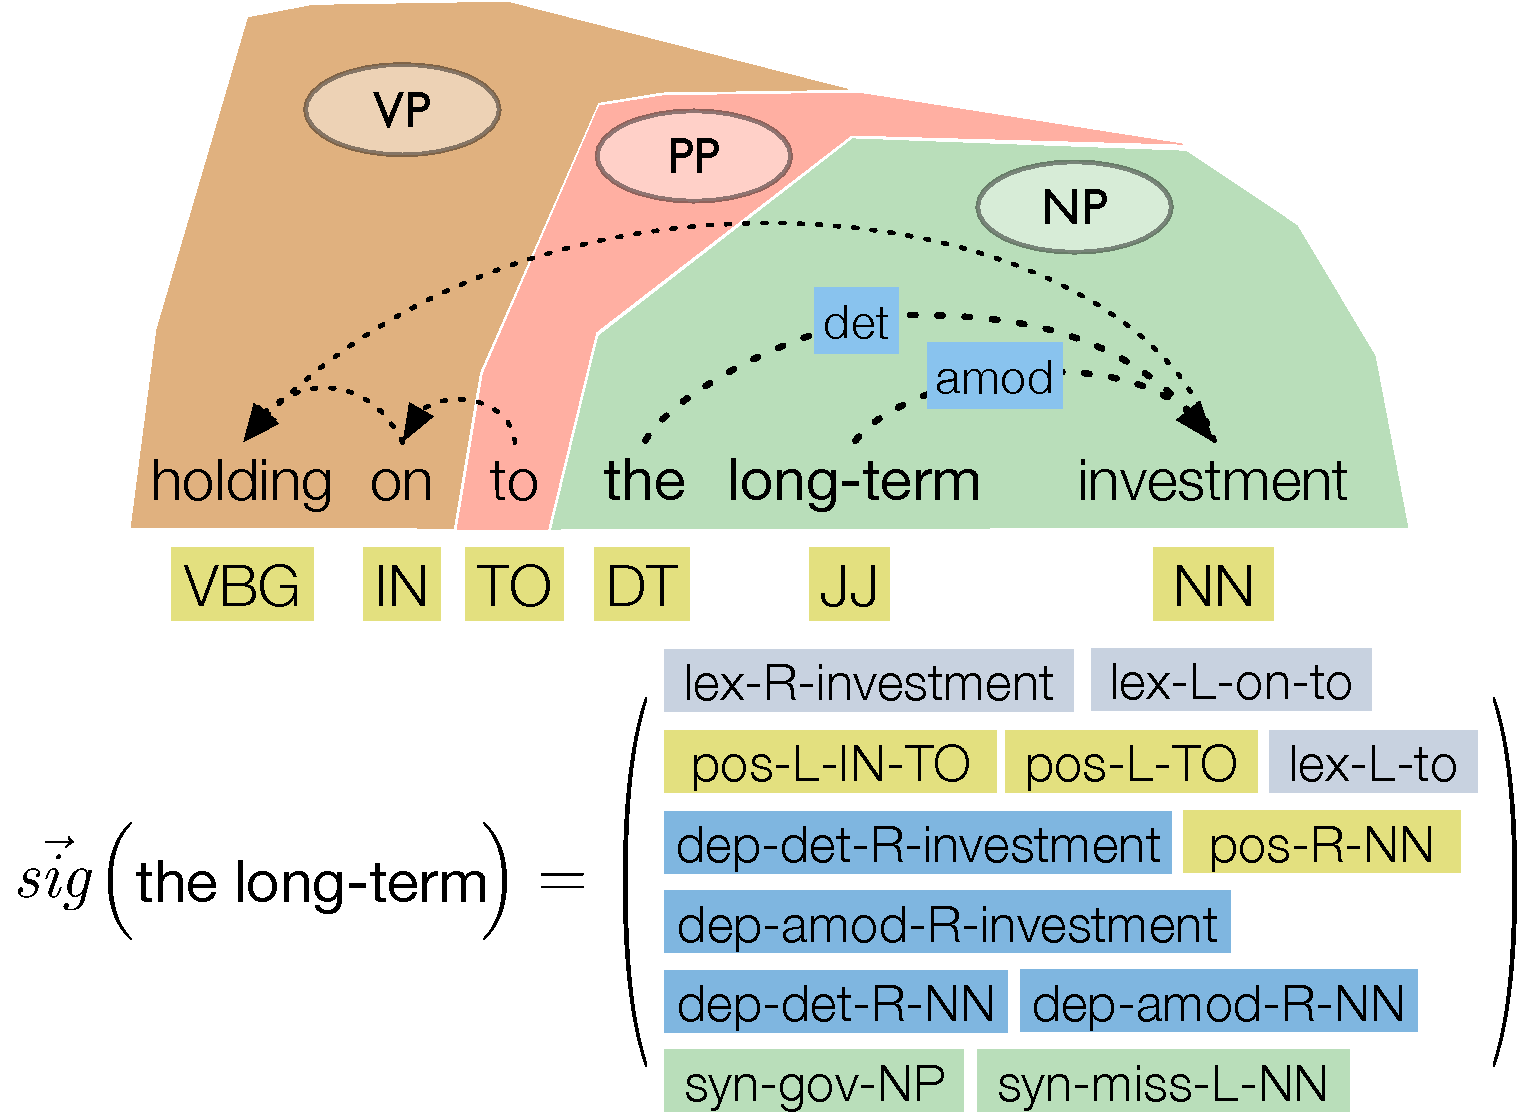
\includegraphics[ width=0.95\linewidth]{figures/rich_context.pdf}
  \caption{\small Here, position-aware lexical and part-of-speech
    $n$-gram features, labeled dependency links , and features
    reflecting the phrase's CCG-style label $\mathit{NP/NN}$ are
    included in the context vector.}\label{fig-rich-context}
\end{figure}

Furthermore, Thrax 2.0 contains a module focused on the extraction of
compact distributional signatures over large datasets. This
\emph{distributional} mode collects contextual features for $n$-gram
phrases, such as words occurring in a window around the phrase, as
well as dependency-based and syntactic
features. Figure~\ref{fig-rich-context} illustrates the feature
space. We then compute a bit signature from the resulting feature
vector via a randomized locality-sensitive hashing projection.  This
yields a compact representation of a phrase's typical context. To
perform this projection Thrax relies on the Jerboa toolkit
\cite{Jerboa}. As part of the PPDB effort, Thrax has been used to
extract rich distributional signatures for 175 million 1-to-4-gram
phrases from the Annotated Gigaword corpus \cite{annotated-gigaword},
a parsed and processed version of the English Gigaword
\cite{Gigaword}.

\begin{table}[t]
  \begin{center}
    \begin{tabular}{|c|r|r|r|r|}
      \hline
    & Disk Space & Extraction Time \\
      \hline
      \hline
      Joshua 4.0 & 245GB & 219 min \\
      \hline
      Joshua 5.0 & 62GB  & 55 min\\
      \hline
      \hline
      Difference & -75\% & -75\% \\
      \hline
    \end{tabular}
  \end{center}
  \caption{Comparing Hadoop's intermediate disk space use and extraction time on a
    De-En Europarl Hiero grammar. Thrax 2.0, bundled with Joshua 5.0,
    is up to 300\% faster and more compact.}
  \label{tab-thrax-speed}
\end{table}




%%%%%%%%%%%%%%%%%%%%%%%%%%%%%%%%%%%%%%%%%%%%%%%%%%%%%%%%%%%%%%%%%
\section{Conclusion}

We present a new iteration of the Joshua machine translation
toolkit. Our system has been extended towards efficiently supporting
large-scale experiments in parsing-based machine translation and
text-to-text generation: Joshua 4.0 supports compactly represented
large grammars with its packed grammars, as well as large language
models via KenLM and BerkeleyLM.We include an implementation of PRO,
allowing for stable and fast tuning of large feature sets, and extend
our toolkit beyond pure translation applications by extending Thrax
with a large-scale paraphrase extraction module.

\paragraph{Acknowledgements}

This research was supported by in part by the EuroMatrixPlus project
funded by the European Commission (7th Framework Programme), and by
the NSF under grant IIS-0713448. Opinions, interpretations, and
conclusions are the authors' alone.

\bibliographystyle{acl2013}
\bibliography{joshua}

\end{document}
